% Generated from selected worked problems in committed QFT-soln sources.
% Source repository: https://github.com/Luca-Yucheng-Jin/QFT-soln
% Source commit: e6cc8da6c7d80431b9a78aa7d9bc7b97f8c261a8
\section{David Tong Statistical Field Theory, Sheet 1: Mean Field Theory}
\markboth{\thesection\quad TONG STATISTICAL FIELD THEORY, SHEET 1}{}

\noindent\textit{These prompts paraphrase David Tong's \emph{Statistical Field Theory},
Example Sheet 1 (October 2018). Problem numbers, starred status, equations, and
guidance follow the \href{https://davidtong.org/pdfs/teaching/statistical-field-theory/99a.pdf}{official sheet}.}

\subsection{Sheet 1, Problem 1: Transfer Matrix for the One-Dimensional Ising Model}

Take $N$ Ising spins with $s_{N+1}=s_1$ and partition function
\begin{equation}
    Z=\sum_{s_1=\pm1}\cdots\sum_{s_N=\pm1}
    \prod_{i=1}^{N}
    \exp\!\left[\beta J s_i s_{i+1}
    +\frac{\beta B}{2}(s_i+s_{i+1})\right].
\end{equation}
Show that $Z=\operatorname{tr}T^N$ for the transfer matrix
\begin{equation}
    T=\begin{pmatrix}
        e^{\beta J-\beta B}&e^{-\beta J}\\
        e^{-\beta J}&e^{\beta J+\beta B}
    \end{pmatrix}.
\end{equation}
\textit{Hint:} Express the $i$th factor as
$T_{s_i,s_{i+1}}=\exp[\beta J s_i s_{i+1}
+\beta B(s_i+s_{i+1})/2]$, with $s_i$ labelling a column and
$s_{i+1}$ a row. Find the two eigenvalues,
\begin{equation}
    \lambda_\pm=e^{\beta J}\cosh(\beta B)
    \pm\sqrt{e^{2\beta J}\cosh^2(\beta B)-2\sinh(2\beta J)},
\end{equation}
and explain why $Z\simeq\lambda_+^N$ as $N\to\infty$. At $B=0$, deduce
that the magnetisation is always zero and that temperature causes no phase
transition in this one-dimensional system.
\begin{solution}
    The partition function can be written as
    \begin{equation}
        Z = \sum_{s_1 = \pm1} \cdots\sum_{s_N = \pm1} T_{s_1,s_2} T_{s_2,s_3}\cdots T_{s_N , s_1} = \operatorname{tr} T^N = \lambda_+^N + \lambda_-^N.
    \end{equation}
    Clearly, $\lambda_+ > \lambda_-$. Therefore, for Large $N$, we can write $Z  \simeq \lambda_+^N$. The magnetisation is given by
    \begin{equation}
        M = \frac{1}{\beta}\frac{\partial \log Z}{\partial B} = \frac{1}{\beta Z}\left[N\lambda_+^{N-1}\frac{\partial \lambda_+}{\partial B} + N\lambda_-^{N-1}\frac{\partial \lambda_-}{\partial B}\right].
    \end{equation}
    Clearly, $\dfrac{\partial \lambda_\pm}{\partial B}\bigg|_{B=0} = 0$, which gives $M \bigg|_{B=0} = 0$. Therefore, there is no second-order phase transition for a one-dimensional system.

\end{solution}

\subsection{Sheet 1, Problem 3: Exact Mean Field Limit of a Long-Range Ising Model}

Let every spin interact with every other spin, including itself, through
\begin{equation}
    E=-B\sum_i s_i-\frac{J}{2N}
    \left(\sum_i s_i\right)\left(\sum_j s_j\right).
\end{equation}
Explain the factor $1/N$. Establish the Gaussian identity
\begin{equation}
    e^{\beta J\alpha^2/(2N)}
    =\sqrt{\frac{N\beta J}{2\pi}}
    \int_{-\infty}^{\infty}dx\,
    e^{-N\beta Jx^2/2+\alpha\beta Jx},
\end{equation}
and use it to express the partition function as
\begin{equation}
    Z=\sqrt{\frac{N\beta J}{2\pi}}
    \int_{-\infty}^{\infty}dx\,e^{-NS(x)},
    \qquad
    S(x)=\frac{\beta Jx^2}{2}
    -\log\!\left[2\cosh\bigl(\beta(B+Jx)\bigr)\right].
\end{equation}
Find the saddle $x_\star$ that dominates at large $N$, up to its prefactor.
Derive its stationarity equation and show that $m=x_\star$.

\begin{solution}
    Since we expect the energy to scale as $N$, while $\sum_i s_i$ also scales as $N$. Therefore, we must have a factor of $1/N$.

    The Gaussian identity is straightforward. Let us define
    \begin{equation}
        \sum_i s_i \equiv \alpha.
    \end{equation}
    Then,
    \begin{equation}
        \begin{aligned}
            Z &= \sum_{\alpha} e^{\beta J \alpha^2/(2N)+\beta B \alpha}\\
            &=\sqrt{\frac{N\beta J}{2\pi}}\sum_\alpha e^{\beta B \alpha}\int_{-\infty}^{\infty}dx\,e^{-N\beta Jx^2/2+\alpha\beta Jx}\\
            &=\sqrt{\frac{N\beta J}{2\pi}}\int_{-\infty}^{\infty}dx\,e^{-N\beta Jx^2/2}\sum_\alpha  \,e^{\beta(B +  Jx)\alpha}\\
            &=\sqrt{\frac{N\beta J}{2\pi}}\int_{-\infty}^{\infty}dx\,e^{-N\beta Jx^2/2} \cdot 2^N\cosh^N\beta(B+ Jx) \\
            &=\sqrt{\frac{N\beta J}{2\pi}}
    \int_{-\infty}^{\infty}dx\,e^{-NS(x)}.
        \end{aligned}
    \end{equation}
    The saddle is given by
    \begin{equation}
        S'(x_\star) = 0 \implies x_\star = \tanh (\beta B + \beta J x_\star),
    \end{equation}
    which satisfies the same equation as $m$ as we have seen. Therefore, we have $m = x_\star$, which means that the long-range Ising model realises the mean field theory exactly.
\end{solution}

\subsection{Sheet 1, Problem 6: Ising and XY Orders in an Anisotropic Spin Model}

At each lattice site put a unit three-vector
$\mathbf s_i=(s_i^x,s_i^y,s_i^z)$ and use
\begin{equation}
    E=-J\sum_{\langle ij\rangle}\mathbf s_i\cdot\mathbf s_j
    +g\sum_i\left[(s_i^z)^2
    -\frac{(s_i^x)^2+(s_i^y)^2}{2}\right],
    \qquad J>0.
\end{equation}
Use mean field reasoning to account for the phase diagram below,

\begin{center}
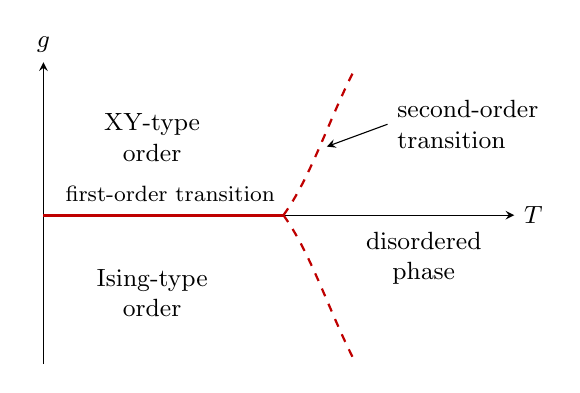
\begin{tikzpicture}[x=1.15cm,y=1.05cm,>=stealth,
    every node/.style={font=\small}]
    \draw[->] (0,-1.8) -- (0,1.85) node[above] {$g$};
    \draw[->] (0,0) -- (5.2,0) node[right] {$T$};
    \draw[red!75!black,very thick] (0,0) -- (2.65,0);
    \draw[red!75!black,thick,dashed] (2.65,0)
        .. controls (2.95,0.45) and (3.15,1.15) .. (3.43,1.75);
    \draw[red!75!black,thick,dashed] (2.65,0)
        .. controls (2.95,-0.45) and (3.15,-1.15) .. (3.43,-1.75);
    \node[align=center] at (1.2,0.94) {XY-type\\order};
    \node[align=center] at (1.2,-0.94) {Ising-type\\order};
    \node[align=center] at (4.2,-0.52) {disordered\\phase};
    \node[above,font=\footnotesize] at (1.4,0.05) {first-order transition};
    \node[align=left,anchor=west] (second) at (3.8,1.1)
        {second-order\\transition};
    \draw[->,thin] (second.west) -- (3.13,0.83);
\end{tikzpicture}
\end{center}

\textit{Hint:} Compare the ground states as $g$ crosses zero at low $T$,
then raise $T$ separately on either side of $g=0$. Detailed path-integral
calculations are unnecessary.
\begin{solution}
    The energy can be rewritten as
    \begin{equation}
        E = -J\sum_{\langle ij\rangle}\mathbf s_i\cdot\mathbf s_j
    +g\sum_i\left[\frac{3}{2}(s_i^z)^2
    -\frac{1}{2}\right].
    \end{equation}

    When $T$ is small and $g > 0 $, to minimise the total energy, the system tend to align while the second term forces them into the $x-y$ plane. Therefore, it is a XY-type order. For $g<0$, energy is minimised when all of the spins is in the $z$-direction and aligned. Hence, it is a Ising-type ordering. Therefore, going from $g<0$ to $g>0$ is a first-order phase transition.

    As the temperature goes up, the system becomes disordered for both $g<0$ and $g>0$. Therefore, a second-order phase transition must have occured.
\end{solution}

\subsection{Sheet 1, Problem 8: Multicritical Scaling and Upper Critical Dimension}

Take
\begin{equation}
    f(m)=\alpha_2m^2+\alpha_{2n}m^{2n},
    \qquad n\in\mathbb Z_+.
\end{equation}
Find $\beta$ from $m\sim(T_c-T)^\beta$ in the ordered phase.
Insert the result into the free energy to show that the heat-capacity
exponent obeys $\alpha=1-2\beta$. Compare this with the
contribution to the free energy from fluctuations in the Gaussian path integral and establish the threshold
$d_c=2n/(n-1)$ above which the mean field term dominates near criticality.
\begin{solution}
    It can be easily obtained that $\beta = 1/(2n-2) <1$. Plugging back into the free energy and noting that $1+2\beta = 2n\beta$, we have
    \begin{equation}
        f \sim \alpha_2^{1+2\beta} \implies c \sim \alpha_2^{2\beta - 1},
    \end{equation}
    and hence $\alpha = 1 - 2\beta$. In the Gaussian path integral, we have
    \begin{equation}
        c \sim |T-T_c|^{-2+d/2}.
    \end{equation}
    Therefore, the critical dimension is
    \begin{equation}
        d_c =\frac{2n}{n-1}.
    \end{equation}
\end{solution}
